\section{Evaluation datasets}
Before the experimental setting testing designed features relevancy is proven in comparison to comprehensive benchmark datasets. There are a few standardized datasets used in the related work \cite{ribeiro_rotating_2017} and are publically available in Comma-Separated Values files. 

\emph{MaFaulDa} dataset combines vibration and acoustic measurements of the shaft in deviating positions and bearings abnormalities.\emph{CWRU dataset} focuses solely on faults in ball bearings. Another less known dataset concerns shaft unbalance, but compared to the previous two, it demonstrates behavior during revolution speed up.  

\subsection{Machinery Fault Database}
MaFaulDa\footnote{MaFaulDa: \url{https://www02.smt.ufrj.br/~offshore/mfs/page_01.html}} is a collection of 1951 multivariate time series for 4 different operational conditions on rotor kit Alignment Balance Vibration Trainer (ABVT)~(Fig.~\ref{fig:mafaulda-simulator}). Each series has 5~seconds in length and is captured at 50 kHz. Vibration signals were obtained with piezoelectric accelerometers with a linear response up to 10~kHz, amplitude range to 490 $m/s^2$, and resolution step of 10.2~mV per $m/s^2$. 

\begin{figure}[h]
\centering
\begin{subfigure}[b]{0.48\textwidth}
	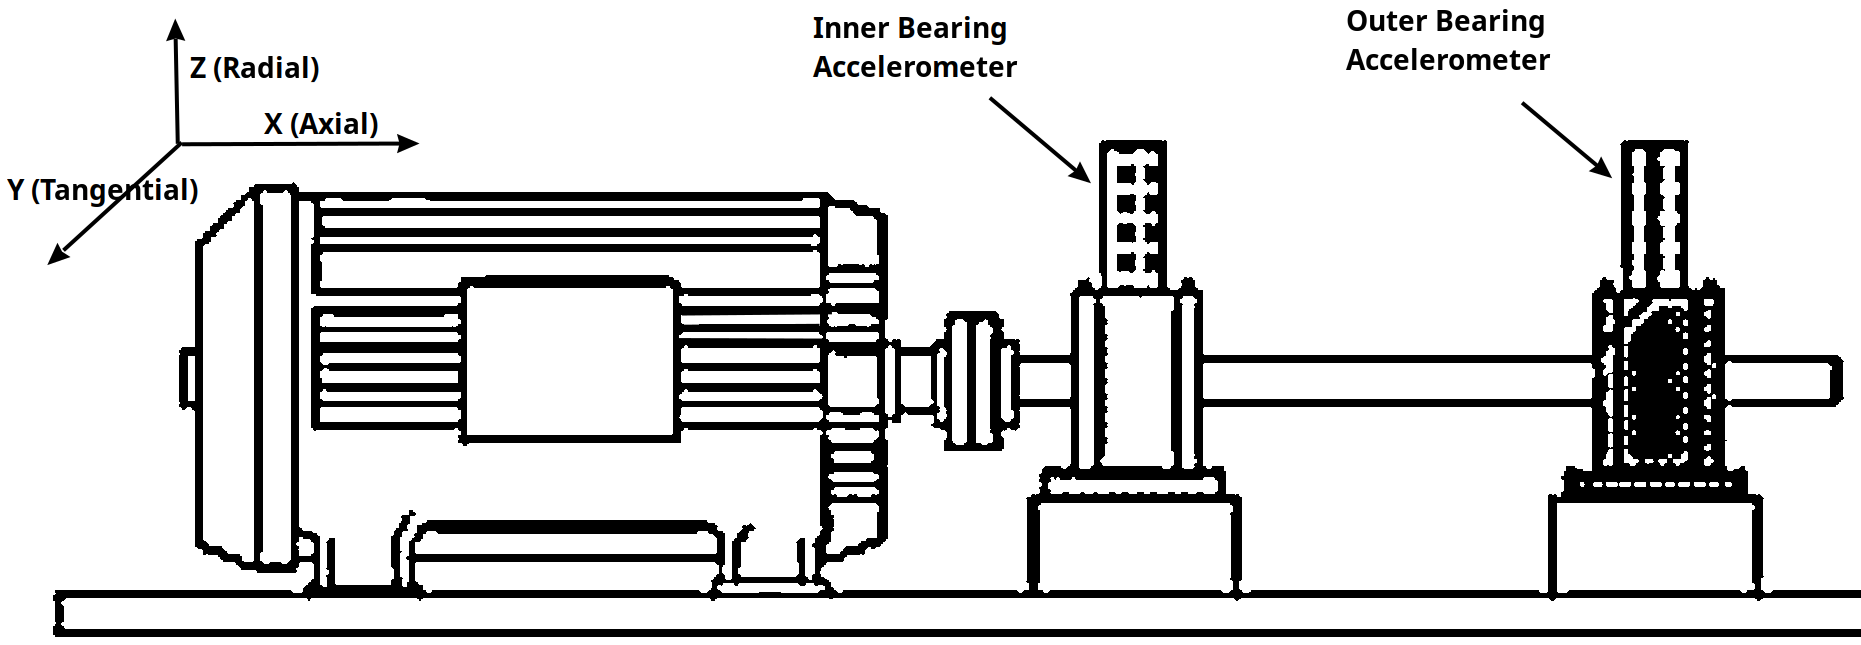
\includegraphics[width=\textwidth]{assets/mafaulda-simulator.png}
	\caption{Schematic diagram \cite{pestana-viana_influence_2016}}
\end{subfigure}
\hfill
\begin{subfigure}[b]{0.48\textwidth}
	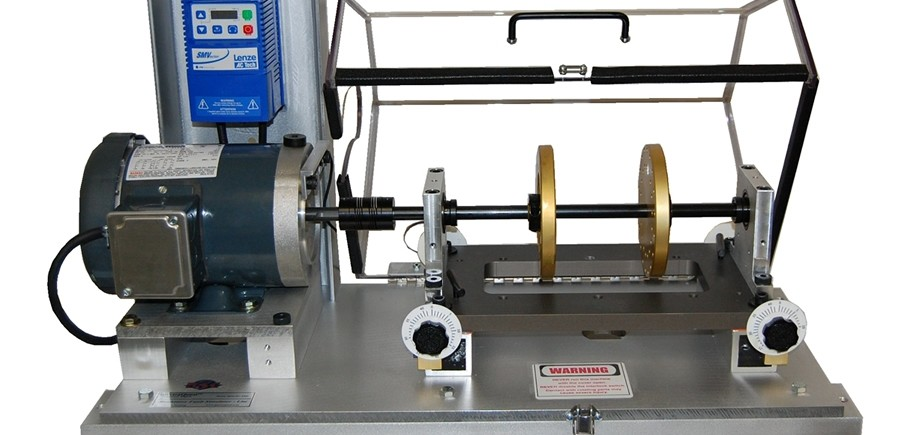
\includegraphics[width=\textwidth]{assets/machinery-fault-simulator.jpg}
	\caption{Mechanical construction \cite{noauthor_spectraquest_nodate}}
\end{subfigure}
\caption{Machinery fault simulator for MaFaulDa}
\label{fig:mafaulda-simulator}
\end{figure}

Observations were conducted in three cardinal axes simultaneously with 2 sets of accelerometers each one associated with one bearing (inner and outer bearings)~(Fig.~\ref{fig:mafaulda-simulator}). Additionally, a magnetic tachometer produced a pulse on shaft turn. The cardioid condenser microphone recorded sound emissions with frequency range 20~Hz - 20~kHz. Sensors were fed into a four-channel dynamic signal acquisition module. 

Columns in dataset are organized as depicted in table~\ref{tab:mafaulda-columns}. Machine rotational speeds were kept constant during a particular measurement, but covered a range from 737 to 3686~rpm with steps of approximately 60 rpm (equiv. 10~Hz - 60~Hz)~\cite{pestana-viana_influence_2016}. The maximal rotational frequency achieved with high unbalance load is 3300 rpm.

\begin{table}[h]
\renewcommand{\arraystretch}{1.2}
\centering
\begin{tabular}{|l|l|}
\hline
\textbf{Columns} & \textbf{Description}                                                                                                                                               \\ \hline
1.               & \begin{tabular}[c]{@{}l@{}}Pulse with modulation of tachometer signal \\ to estimate rotation frequency  (in TTL levels)\end{tabular}                              \\ \hline
2., 3., 4.       & \begin{tabular}[c]{@{}l@{}}Underhang bearing accelerometer \\ (inner - between the rotor and motor)\\ - axial, radial, tangential direction\end{tabular}           \\ \hline
5., 6., 7.       & \begin{tabular}[c]{@{}l@{}}Overhang  bearing accelerometer \\ (Outer - outside most position after the rotor)\\ - axial, radial, tangential direction\end{tabular} \\ \hline
8.               & Microphone                                                                                                                                                         \\ \hline
\end{tabular}
\caption{MaFaulDa columns' descriptions}
\label{tab:mafaulda-columns}
\end{table}

This database contains normal operating conditions, faults out of unbalance, horizontal and vertical shaft misalignment, and three types of faulty bearings in inner and outer positions: outer track, inner track, rolling elements~\cite{pestana-viana_influence_2016}.
\begin{itemize}
\itemsep0pt
\item \textbf{Normal} conditions are baseline without the adverse effect of fault in 49 different rotation speeds. 
\item \textbf{Unbalance} shaft time series uses 8 unbalancing weights from 6 to 35 grams and varying 45 - 49 speeds for each weight adding to 333 mass unbalance loads. 
\item \textbf{Vertical misalignement} set is comprised of 50 signals each (or 51 in one instance) obtained under displacements: 0.51, 0.63, 1.40, 1.90, 1.27, 1.78 mm.
\item \textbf{Horizontal misalignement} signals were recorded under displacements: 0.50, 1.00, 1.50, 2.00 mm, each with 49 different speeds (or 50 in one instance)~\cite{pestana-viana_influence_2016}.
\item \textbf{Bearing faults} are unnoticable without unbalance. Therefore, weights of 6, 20, and 35 grams were attached to induce a detectable effect. Each unbalance mass was combined with cage, outer race, and ball faults at multiple rotation speeds, usually at 50 different speeds.
\end{itemize}

%TODO
\subsection{Case Western Reserve University bearing database}
(CWRU) 
2 HP (1.492 kW) Reliance Electric motor \footnote{\url{https://engineering.case.edu/bearingdatacenter/download-data-file}}
Bearings - Inner, Outer
12 kHz, 48 kHz
fan and drive end bearings
Fault diameters of 7 mils, 14 mils, 21 mils, 28 mils, and 40 mils (1 mil=0.001 inches) in diameter were introduced separately at the inner raceway, rolling element (i.e. ball) and outer raceway. 

% Faults ranging from 0.007 inches in diameter to 0.040 inches in diameter were introduced separately 
% at the inner raceway, rolling element (i.e. ball) and outer raceway. 
%Faulted bearings were reinstalled into the test motor and vibration data
%was recorded for motor loads of 0 to 3 horsepower (motor speeds of 1797 to 1720 RPM).

% Feature-based performance of SVM and KNN classifiers for diagnosis of rolling element bearing faults
\cite{jamil_feature-based_2021}

\begin{figure}[h]
\centering
\begin{subfigure}[b]{0.48\textwidth}
	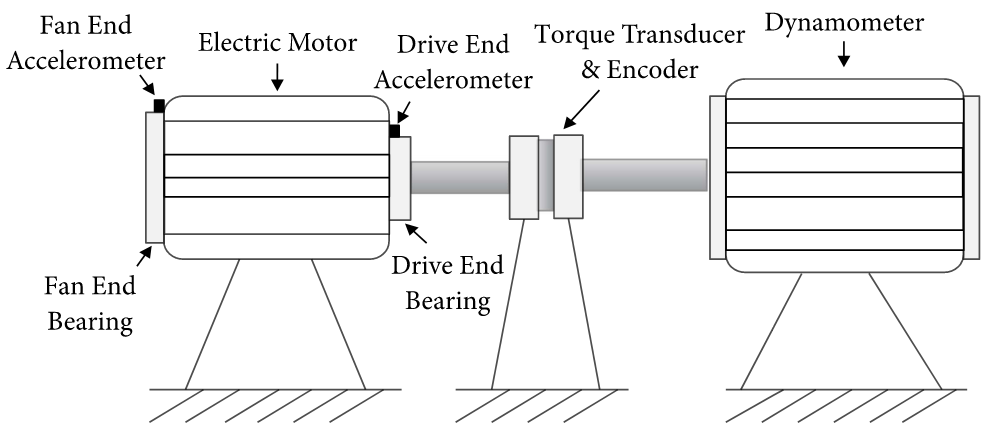
\includegraphics[width=\textwidth]{assets/cwru-test-stand-2.png}
	\caption{Schematic diagram \cite{song_bearing_2022}}
\end{subfigure}
\hfill
\begin{subfigure}[b]{0.48\textwidth}
	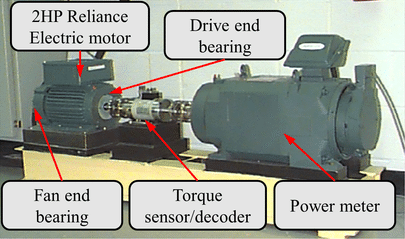
\includegraphics[width=\textwidth]{assets/cwru-test-stand.png}
	\caption{Mechanical construction \cite{yuhong_new_2021}}
\end{subfigure}
\caption{CWRU machine apparatus}
\label{fig:cwru-simulator}
\end{figure}



\subsection{Unbalance on rotating shaft}
Shaft -  unbalances of different sizes \footnote{\url{https://www.kaggle.com/datasets/jishnukoliyadan/vibration-analysis-on-rotating-shaft}}

% Unbalances of different sizes was recorded. Sampling rate =  4096 Hz
% 4 different unbalance strengths were recorded as well as one dataset with the unbalance holder without additional weight (i.e. without unbalance). 
%The rotation speed was varied between approx. 630 and 2330 RPM in the development datasets 
% and between approx. 1060 and 1900 RPM 

%Columns:
% V_in =  The input voltage to the motor controller V_in (in V)
% Measured_RPM  = The rotation speed of the motor (in RPM; computed from speed measurements using the DT9837)
% Vibration_[1 - 3]      : The signal from the 1.,2.,3. vibration sensor

% (“0” = no unbalance, “4” = strong unbalance), (“D” = development or training, “E” = evaluation)
% Radius in mm = 0, 14, 18.5, 23, 23
% Mass 3.3 g (0 ... 3), 6.6 g in 4

\begin{figure}[h]
\centering
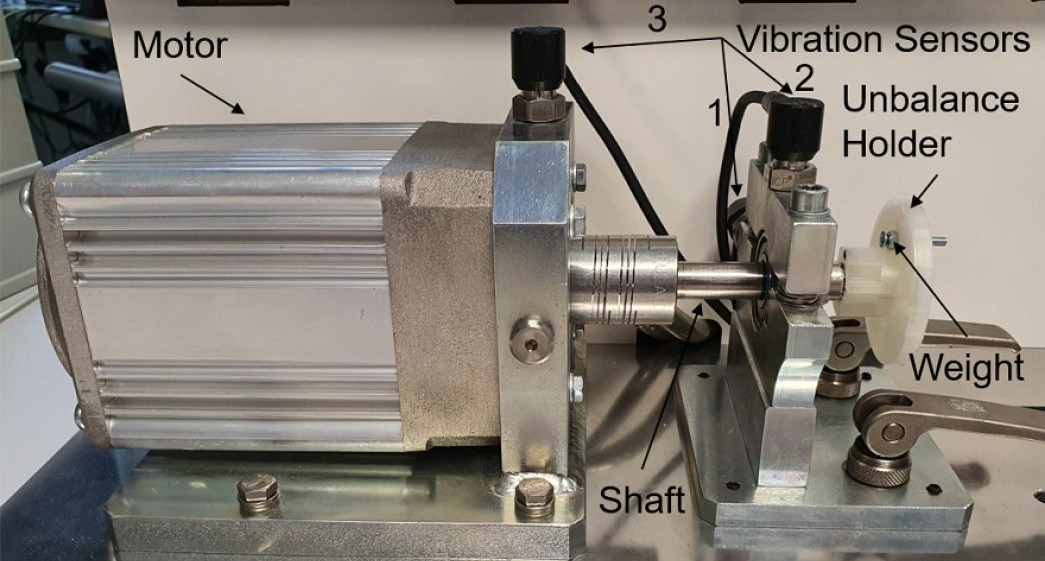
\includegraphics[width=0.7\textwidth]{assets/rotating-shaft.jpg}
\caption{Motor driving shaft in unbalance measurement \cite{mey_machine_2020}}
\label{fig:rotating-shaft}
\end{figure}

% Machine Learning-Based Unbalance Detection of a Rotating Shaft Using Vibration Data
\cite{mey_machine_2020}

